\documentclass[12pt, a4paper]{article}
\usepackage[spanish]{babel}             % Español para los nombres
\usepackage[utf8]{inputenc}             % Codificación de entrada
\usepackage[T1]{fontenc}                % Codificación de fuente (escribir castellano)
\usepackage{lmodern}                    % Fuente (la default no es compatible con castellano)
\usepackage{csquotes}                   % Para comillas y otras anotaciones del castellano
\usepackage{fancyhdr}                   % Encabezado y Pie de pagina
\usepackage{tocloft}                    % Puntos en los índices

\usepackage{url}                        % 
\usepackage{hyperref}                   % Links y referencias dentro del texto
\usepackage{nameref}                    % Para poder referenciar por nombre
\usepackage{acronym}                    % Para incluir las listas de abreviaturas
\usepackage{multicol}                   % Permite crear espacios con columnas verticales
\usepackage{booktabs} % Para mejores líneas horizontales en tablas
\usepackage{parskip}                    % Eliminar sangrado y añadir espacio entre párrafos
\usepackage{titlesec}                   % Crear subsubsub secciones
\usepackage{amsmath}                    % Funciones para ecuaciones
\usepackage{blkarray}                   % Matrices con anotaciones
\usepackage{algorithm}                  % Algoritmos con formalismos
\usepackage{algpseudocode}              % También para algoritmos
\usepackage{listings}                   % Para insertar codigo

\usepackage{array}                      % Para personalizar columnas de tabla
\usepackage{tabularx}                   % Para tablas de ancho variable

\usepackage{graphicx}                   % Para incluir imágenes
\usepackage{subcaption}                 % Subfiguras
\usepackage[table]{xcolor}              % Definir y utilizar colores
\usepackage{tikz}                       % Dibujar formas, figuras, rectas, intersecciones...
\usepackage[absolute,overlay]{textpos}  % Posición absoluta para textos
\usepackage{geometry}                   % Para controlar los márgenes

\usepackage{float}
\usepackage{soul}                       % Para highligths \hl
\usepackage{lipsum} 

\usepackage[backend=biber, sorting=none]{biblatex} % Referencias (bibliografía / webgrafía)
\selectlanguage{spanish}                % Seleccionar español
\bibliography{referencias}              % Incluir el archivo de referencias

\setlength{\emergencystretch}{3em}

% Definición de nombres
%\printbibliography[title={Bibliografía}]
\renewcommand{\cftsecleader}{\cftdotfill{\cftdotsep}} 
\renewcommand{\spanishtablename}{Tabla}
\renewcommand{\spanishlisttablename}{Índice de tablas}
\newcommand{\estudiante}{García Justel, Alan}
\newcommand{\director}{}
\newcommand{\master}{INGENIERÍA COMPUTACIONAL Y SISTEMAS INTELIGENTES}
\newcommand{\titulo}{PREANOTACIÓN DE ESCENAS VEHICULARES CON SEGMENTACIÓN SEMÁNTICA EN VISTA TOP-DOWN}
\newcommand{\portada}{images/shared/no_signal.jpg}
\newcommand{\curso}{2023-2024}

% Definición de Macros
\newcommand*{\fullref}[1]{\hyperref[{#1}]{\autoref*{#1} \nameref*{#1}}} % One single link

\newcommand{\aclink}[1]{% Crear links a acronimos
  \ifcsdef{ac@#1}{%
    \ifcsdef{mark@#1}{%
      \hyperlink{acro:#1}{\acs{#1}}%
    }{%
      \hyperlink{acro:#1}{\ac{#1}}%
      \expandafter\gdef\csname mark@#1\endcsname{}%
    }%
  }{%
    \ac{#1}%
    \expandafter\gdef\csname mark@#1\endcsname{}%
  }%
}

% Notas en Figuras
\newcommand\fnote[1]{\captionsetup{width=0.8\linewidth, font=footnotesize}\caption*{#1}}

% Estilos de listings
% Configuración del estilo para resaltar el código de ROS
\lstdefinestyle{ros}{
    backgroundcolor=\color{white}, % Cambiar el color de fondo
    basicstyle=\small\ttfamily, % Texto más pequeño
    breaklines=true,
    language=C,
    morekeywords={int32, float64},
    keywordstyle=\color{blue},
    commentstyle=\color{green!40!black},
    stringstyle=\color{red},
    breakatwhitespace=false,         
    breaklines=true,                 
    captionpos=b,                    
    keepspaces=true,                 
    numbers=left,                    
    numbersep=5pt,                  
    showspaces=false,                
    showstringspaces=false,
    showtabs=false,                  
    tabsize=2
}

% Crear subsubsub secciones
\titleclass{\subsubsubsection}{straight}[\subsection]
\newcounter{subsubsubsection}[subsubsection]
\renewcommand\thesubsubsubsection{\thesubsubsection.\arabic{subsubsubsection}}
\renewcommand\theparagraph{\thesubsubsubsection.\arabic{paragraph}} % optional; useful if paragraphs are to be numbered

\titleformat{\subsubsubsection}
  {\normalfont\normalsize\bfseries}{\thesubsubsubsection}{1em}{}
\titlespacing*{\subsubsubsection}
{0pt}{3.25ex plus 1ex minus .2ex}{1.5ex plus .2ex}
\makeatletter
\renewcommand\paragraph{\@startsection{paragraph}{5}{\z@}%
  {3.25ex \@plus1ex \@minus.2ex}%
  {-1em}%
  {\normalfont\normalsize\bfseries}}
\renewcommand\subparagraph{\@startsection{subparagraph}{6}{\parindent}%
  {3.25ex \@plus1ex \@minus .2ex}%
  {-1em}%
  {\normalfont\normalsize\bfseries}}
\def\toclevel@subsubsubsection{4}
\def\toclevel@paragraph{5}
\def\toclevel@paragraph{6}
\def\l@subsubsubsection{\@dottedtocline{4}{7em}{4em}}
\def\l@paragraph{\@dottedtocline{5}{10em}{5em}}
\def\l@subparagraph{\@dottedtocline{6}{14em}{6em}}
\makeatother
\setcounter{secnumdepth}{4}
\setcounter{tocdepth}{4}



% Encabezado y Pie de pagina
\pagestyle{fancy}                       % Estilo de las páginas
\fancyhf{}
\fancyhead[L]{Trabajo Fin de Máster}
\fancyhead[R]{\leftmark}
\fancyfoot[L]{UPV/EHU}
\fancyfoot[R]{\thepage}
\renewcommand{\footrulewidth}{0.4pt} % Línea horizontal en el pie de página
\setlength{\headheight}{15.5pt}

% Definición de colores
\definecolor{ehu_blue}{HTML}{376092}
\definecolor{link_color}{HTML}{36AEB4}
\definecolor{reference_color}{HTML}{0F3133}
\definecolor{cite_color}{HTML}{ff7f42}
\definecolor{table_gray}{HTML}{C0C0C0}
\definecolor{table_red}{HTML}{fb4952}


% Incluye todas las entradas del archivo .bib en la bibliografía
\nocite{*}

% Configuración de hyperref para diferentes tipos de enlaces
\hypersetup{
    colorlinks=true,
    linkcolor=reference_color,
    citecolor=cite_color,
    filecolor=link_color,
    urlcolor=link_color,
}

% #########################################################################
% #                                  TFM                                  #
% #########################################################################
\begin{document}
\newgeometry{bottom=2cm}

\begin{titlepage}
    % Logo de la universidad
    \begin{textblock*}{\textwidth}(10cm,0cm)
        
\includegraphics[width=7.5cm, height=3cm]{images/shared/Logo_EHU.jpg}
    \end{textblock*}
    
    % Franja azul
    \begin{tikzpicture}[remember picture, overlay]
        \fill[ehu_blue] (current page.north west) ++ (0,-3.01cm) rectangle (\paperwidth,-3cm);
    \end{tikzpicture}
    
    \begin{textblock*}{\paperwidth}(\dimexpr\parindent+\oddsidemargin+3em\relax,3.5cm)
        \begin{minipage}{\dimexpr\linewidth-7.5cm\relax}
            \color{white}
            \noindent\rule{\linewidth}{0cm}
            \textsf{ {\large MÁSTER EN \master}}
            \newline
            \newline \newline
            \textsf{\textbf{ {\Huge TRABAJO FIN DE MÁSTER }}}
        \end{minipage}
    \end{textblock*}
    
    % Título del trabajo
    \vspace*{3.5cm}
    \begin{minipage}{\linewidth}
        \setlength{\baselineskip}{1.7\baselineskip}
        \centering
        \textsf{ \textbf{ {\LARGE \titulo }}}
    \end{minipage}

    % Foto de portada
    \vspace*{0.5cm}
    \begin{figure}[H]
        \centering
        \includegraphics[width=10cm, height=8cm]{\portada}
    \end{figure}

    % ODS
    \vspace*{1cm}
    % \begin{figure}[h]
    % \centering
    %     \begin{subfigure}[b]{0.135\textwidth}
    %         \includegraphics[width=2cm, height=2cm]{images/iconos_ods/03.png}
    %     \end{subfigure}
    %     \begin{subfigure}[b]{0.135\textwidth}
    %         \includegraphics[width=2cm, height=2cm]{images/iconos_ods/04.png}
    %     \end{subfigure}
    %     \begin{subfigure}[b]{0.135\textwidth}
    %         \includegraphics[width=2cm, height=2cm]{images/iconos_ods/05.png}
    %     \end{subfigure}
    %     \begin{subfigure}[b]{0.135\textwidth}
    %         \includegraphics[width=2cm, height=2cm]{images/iconos_ods/07.png}
    %     \end{subfigure}
    %     \begin{subfigure}[b]{0.135\textwidth}
    %         \includegraphics[width=2cm, height=2cm]{images/iconos_ods/08.png}
    %     \end{subfigure}
    %     \begin{subfigure}[b]{0.135\textwidth}
    %         \includegraphics[width=2cm, height=2cm]{images/iconos_ods/09.png}
    %     \end{subfigure}
    %     \begin{subfigure}[b]{0.135\textwidth}
    %         \includegraphics[width=2cm, height=2cm]{images/iconos_ods/12.png}
    %     \end{subfigure}
    % 
    %     \label{fig:ods-iconos}
    % \end{figure}
    
    % Estudiante
    \vspace{0.2cm}
    \noindent {\footnotesize \textbf{Estudiante:} \estudiante}
    \newline
    \noindent\makebox[\linewidth]{\rule{\textwidth}{0.4pt}} % Línea horizontal

    % Director
    \nopagebreak
    \vspace{0.3cm}
    \nopagebreak
    \noindent {\footnotesize \textbf{Director/Directora:} \director }

    % Espacio para firmas
    \vspace{0.5cm} % Espacio entre texto "Director/Directora" y espacio para firmas
    \noindent 
    \makebox[0.4\linewidth]{\hrulefill}
    \hspace{0.2\linewidth}
    \makebox[0.4\linewidth]{\hrulefill}

    % Curso y Fecha
    \vspace{0.1cm}    
    \noindent {\footnotesize \textbf{Curso: } \curso \hfill \textbf{Fecha:} \today }
\end{titlepage}

\restoregeometry
\setcounter{figure}{0} % Incluimos el título

% \newpage % BORRAR EN LA VERSIÓN FINAL
% \input{notas}

\newpage
\markboth{Resumen}{Resumen}
\begin{itshape}
    \textbf{Resumen:} \\
    
    \textbf{Palabras Clave: }
\end{itshape}
\newpage

\begin{itshape}
    \textbf{Abstract:} \\

    \textbf{Key Words: }
\end{itshape}
\newpage

\begin{itshape}
    \textbf{Laburpena:} \\

    \textbf{Gako-hitzak: }
\end{itshape}

\newpage

 % Incluimos el resumen tri-lingüe

% Índices
\tableofcontents\thispagestyle{empty}\newpage
\listoffigures\thispagestyle{empty}\newpage
\listoftables\thispagestyle{empty}\newpage

% Abreviaturas
\section*{Abreviaturas}
\markboth{Abreviaturas}{Abreviaturas}
\addcontentsline{toc}{section}{Abreviaturas}
%\begin{multicols}{2} % Si se quieren en dos columnas verticales
\begin{acronym}[ADAS]  % El acrónimo más largo
    \acro{TFM}{Trabajo Fin de Máster}
    \acro{ADS}{Automated Driving Systems}
    \acro{ADAS}{Advanced Driving Assistance Systems}
    \acro{SAE}{Society of Automotive Engineers}
    \acro{V2I}{Vehicle-to-Infrastructure}
    \acro{V2X}{Vehicle-to-Everything}
    \acro{BEV}{bird's-eye-view}
    \acro{LiDAR}{Light Detection and Ranging}
\end{acronym}
%\end{multicols}

 % Marcar como visto (No te desglosa el acrónimo)
 % Provoca warnings pero funciona :)
\acused{ADAS}
\acused{LiDAR}
\newpage

\section{Introducción}
% ================================================
% =                INTRODUCCIÓN                  =
% ================================================ 
bla bla bla

\section{Estado del arte}
% ================================================
% =              STATE OF THE ART                =
% ================================================ 
Actualmente, la industria de la automoción está impulsando el desarrollo de los \aclink{ADS} con la promesa de reducir los accidentes en carretera y minimizar los costes tanto humanos como económicos que estos suponen \cite{survey_AutomatedDriving1}. Sin embargo, a pesar de que la conducción automatizada haya incrementado recientemente la atención de la industria por el auge del DeepLearning y la visión por ordenador, lo cierto es que lleva presente más de 20 años.

Algunas de las primeras competiciones de conducción automatizada, como los DARPA Challenges en 2003 y 2005 o el Grand DARPA Urban challenge de 2007, impulsaron enormemente el desarrollo de los \aclink{ADS}, atrayendo la atención tanto de empresas tecnológicas como del sector automotriz \cite{survey_AutomatedDriving2}. Este avance ha sido acompañado por la definición de buenas prácticas y procesos de estandarización para garantizar la seguridad y fiabilidad de los \aclink{ADS}. En este contexto, la \aclink{SAE} ha establecido una escala progresiva de automatización, desde el nivel 0 (sin automatización) hasta el nivel 5 (automatización total), definiendo el grado de intervención del conductor en cada etapa \cite{AD_Technical_Standards}. 

Hoy en día, la mayoría de los vehículos incorporan sistemas avanzados de asistencia a la conducción \aclink{ADAS}, que operan en los niveles \aclink{SAE} 2 y 3. No obstante, ya existen \aclink{ADS} de nivel 4, como los desarrollados por Waymo y Cruise para robotaxis, o los autobuses autónomos desplegados en algunas ciudades, cuyos sistemas están diseñados para gestionar el fallback de manera autónoma, sin necesidad de intervención humana \cite{fallback_strategy}.

Este desarrollo ha llevado a la creación de distintas estrategias y arquitecturas para los \aclink{ADS}. En los últimos años, ha habido grandes avances en soluciones \mbox{End-to-End}, que combinan técnicas de aprendizaje profundo y aprendizaje por refuerzo para obtener las acciones de control del vehículo partiendo diréctamente de los datos de los sensores \cite{end_to_end_driving}. Sin embargo, la mayoría de los enfoques optan por soluciones modulares más tradicionales, que dividen el problema de la conducción automatizada en \mbox{sub-tareas} específicas, integrando soluciones de campos como la robótica, visión por ordenador, deep learning y control automático.

En el contexto de las arquitecturas modulares, la adopción de buenas prácticas ha facilitado la categorización de estas \mbox{sub-tareas} en tres grupos principales \cite{machines5010006}\cite{functional_architectures}: 
\begin{itemize}
    \item Percepción, que se refiere a la capacidad del sistema autónomo para recolectar información del entorno y extraer conocimiento relevante, como la ubicación de obstáculos, señales de tráfico y la localización del vehículo.
    \item Planificación del comportamiento, que consiste en tomar decisiones para alcanzar los objetivos del vehículo, como llegar de un punto a otro evitando obstáculos y optimizando la trayectoria.
    \item Ejecución de movimientos, que se refiere a la capacidad del vehículo para ejecutar las acciones planificadas por el sistema, controlando la dirección, velocidad y maniobras necesarias.
\end{itemize}
Además, estas \mbox{sub-tareas} interactúan entre sí, con el hardware del vehículo y con sistemas de comunicación como \aclink{V2I} o \aclink{V2X} en el caso de los vehículos conectados.

\begin{figure}[H]
    \centering
    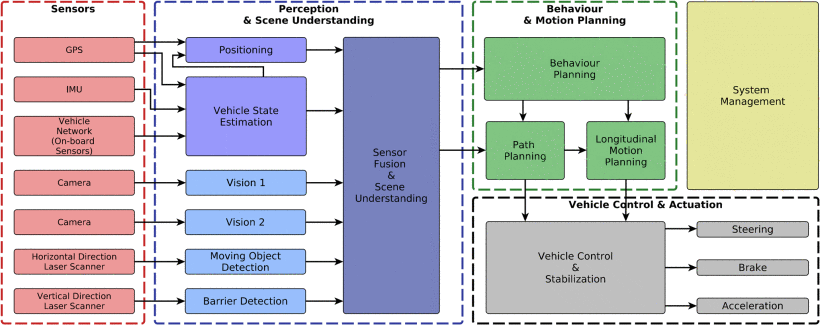
\includegraphics[width=\linewidth]{images/sota/ADS_information_flow.png}
    \label{sota_ads_information_flow}
    \caption{Arquitectura modular de un ADS. TEMPORAL!!!}
\end{figure}

En este tipo de arquitecturas, un error en una \mbox{sub-tarea} puede propagarse y afectar el desempeño de otras, comprometiendo así el funcionamiento del sistema. Esto es especialmente crítico en el módulo de percepción, ya que la calidad de la información obtenida impacta directamente en tareas posteriores como la localización, el mapeo y la planificación. Por ello, garantizar sistemas de percepción robustos es fundamental para el rendimiento y la seguridad de los \aclink{ADS}.

Dos de las tareas principales de los sistemas de percepción en los \aclink{ADS} son la detección 3D de objetos y la segmentación en \aclink{BEV}. La detección 3D de objetos es una de las tareas más relevantes y comúnmente se basa en nubes de puntos obtenidas mediante sensores LiDAR. En ausencia de LiDAR, una alternativa es la detección 3D multi-cámara, que busca predecir cajas delimitadoras 3D en un sistema de coordenadas \aclink{BEV} utilizando únicamente imágenes monoculares. Por otro lado, la segmentación en \aclink{BEV} tiene como objetivo realizar una segmentación semántica del entorno, identificando áreas transitables y delimitaciones de carril en el marco de referencia del vehículo. A diferencia de la detección de objetos, la segmentación en \aclink{BEV} permite una predicción densa de clases estáticas del entorno, lo que resulta clave para la construcción de mapas locales, estimación del comportamiento de agentes y downstream tasks como la planificación del comportamiento del \aclink{ADS}. \hl{Añadir referencias.}

% Parrafo conector que no se me ocurre nada
Este \aclink{TFM} se desarrolla en el contexto de la segmentación semántica en \aclink{BEV}\dots \hl{COMPLETAR.}


\subsection{Semantic segmentation}
\lipsum[2-4] % TODO

\subsection{BEV semantic segmentation}

% TODO: Esto es una piedra de ChatGPT y hay varios errores. Reescribir todo.
%       Alguna imagen no estaría de más.
%

Traditional methods (3D\_Traffic\_Scene\_Understanding) estimate local BEV maps using multi-camera input under the flat-ground assumption, applying Inverse Perspective Mapping (IPM). However, these methods require accurate camera parameters, which has led to research focusing on camera parameter estimation for BEV transformation (BEV\_Params\_Estimation1, BEV\_Params\_Estimation2).

Cam2BEV applies IPM to transform multi-camera input images into BEV space and refines the representation using homographies fed into the model. To handle occlusions, Cam2BEV introduces an additional semantic class that explicitly marks occluded areas from all vehicle-mounted cameras, improving the final BEV estimation.

HDMapNet generates high-definition semantic maps from multi-camera input by employing a feature projection module that transforms image features into BEV space. It models the 3D environment implicitly using an MLP and explicitly incorporates camera extrinsic parameters to project image-space features correctly into BEV. The model first extracts image features with a shared MLP backbone, transforms them into the camera coordinate system, and then projects them into BEV using camera extrinsics.

PYVA introduces a cross-view transformer that projects features from the front-view domain to the BEV domain. While similar to HDMapNet, PYVA differs in that it does not rely on camera parameters in the second transformation stage. Instead, it employs a GAN-based framework to manage occlusions, making it applicable for monocular settings but less suitable for multi-camera fusion.

Other approaches propose different architectures for BEV semantic segmentation. VPN introduces a two-layer MLP for multi-camera feature fusion, followed by a decoder for semantic segmentation in indoor environments. LSS presents a unified framework that lifts 2D images into 3D space by learning an implicit depth distribution, making it effective for end-to-end motion planning. M²BEV transforms 2D image features into 3D voxels along projection rays to generate an efficient BEV representation that supports tasks such as semantic segmentation and 3D object detection. BEVFormer, on the other hand, employs a transformer-based approach that aggregates spatial-temporal features from multi-view cameras and historical BEV frames, enhancing occlusion reasoning.

MonoLayout tackles occlusion estimation by employing a standard encoder-decoder framework combined with adversarial training, enabling it to predict amodal layouts of the driving scene. BEVFormer similarly enhances occlusion reasoning by leveraging attention mechanisms to fuse multi-view spatial-temporal features from historical BEV maps.

Several methods integrate multiple sensor modalities to improve BEV representations. FishingNet extends VPN by incorporating data from additional sensors, while HDMapNet also supports LiDAR fusion, allowing for a more detailed understanding of the driving environment.

To the best of our knowledge, Cam2BEV is the closest approach to this thesis. However, our work differs in several key aspects. Instead of applying semantic segmentation after transforming images into BEV space, we study whether training a segmentation model directly on BEV images improves the representation of planar elements compared to the traditional segmentation-first-then-IPM approach. Furthermore, we treat occupancy and occlusion mask generation as a post-processing step applied to BEV semantic segmentation. This is integrated into a pre-annotation pipeline for vehicle scenes, contributing to advancements in monocular 3D object detection.



% \newpage
% \section*{Agradecimientos}
% % ==========================================================
% =                    AGRADECIMIENTOS                     =
% ==========================================================
\label{agradecimiento}
Lore ipsum...
% 
% \newpage
% \section{Anexos}
% % ==========================================================
% =                         ANEXOS                         =
% ==========================================================
\phantomsection
\subsection{Dummy section} 
Lore ipsum...



\newpage\printbibliography
\addcontentsline{toc}{section}{Referencias}

\end{document}
